\documentclass[conference]{IEEEtran}
\IEEEoverridecommandlockouts
% The preceding line is only needed to identify funding in the first footnote. If that is unneeded, please comment it out.
\usepackage{cite}
\usepackage{amsmath,amssymb,amsfonts}
\usepackage{algorithmic}
\usepackage{graphicx}
\usepackage{textcomp}
\usepackage{xcolor}
\usepackage{booktabs}
\usepackage{tabularx}
\usepackage{multirow}
\usepackage{siunitx}    % 用于处理 \SI{50}{m} 等单位和数字
\usepackage{diagbox}
\def\BibTeX{{\rm B\kern-.05em{\sc i\kern-.025em b}\kern-.08em
    T\kern-.1667em\lower.7ex\hbox{E}\kern-.125emX}}
\begin{document}

\title{OpenCOOD-Air: Prompting Heterogeneous Ground-Air Collaborative Perception with Spatial Conversion and Offset Prediction\\
}

\author{Xianke Wu$^{1}$, Songlin Bai$^{2}$, Chengxiang Li$^{3}$, Zhiyao Luo$^{4}$, Yulin Tian$^{5}$, Fenghua Zhu$^{4}$, Yisheng Lv$^{4}$, Yonglin Tian$^{4}$$^{\dagger}$% <-this % stops a space
\thanks{$^{\dagger}$Corresponding author: Yonglin Tian. {\tt\small yonglin.tian@ia.ac.cn}}%

\thanks{$^{1}$Xianke Wu is with the School of Computer Science, Beijing University
of Posts and Telecommunications, Beijing 100876, China. {\tt\small sinclairwww@bupt.edu.cn}}%

\thanks{$^{2}$Songlin Bai is with the Meituan Group, Beijing 100102, China. {\tt\small baisonglin@meituan.com}}%

\thanks{$^{3}$Chengxiang Li is with the School of Information and Intelligent Engineering, University of Sanya, Sanya 572000, Hainan Province, China. {\tt\small chengxiangli@sanyau.edu.cn}}%

\thanks{$^{4}$Zhiyao Luo, Fenghua Zhu, Yisheng Lv, Yonglin Tian are with the Institute of Automation, Chinese Academy of Sciences, Beijing 100190, China. {\tt\small luozhiyao2024@ia.ac.cn, fenghua.zhu@ia.ac.cn, yisheng.lv@ia.ac.cn, yonglin.tian@ia.ac.cn} }%

\thanks{$^{5}$Yulin Tian is with the College of Mechanical and Electrical Engineering, Zhoukou Normal University, Zhoukou 466001, Henan Province, China. {\tt\small tianyulin@zknu.edu.cn}}%


}

% \begin{icmlauthorlist}
%     \icmlauthor{Jianli Sun}{casia}
%     \icmlauthor{Bin Tian}{casia}
%     \icmlauthor{Qiyao Zhang}{bit}
%     \icmlauthor{Chengxiang Li}{syu}
%     \icmlauthor{Zihan Song}{hnu}
%     \icmlauthor{Zhiyong Cui}{bhu}
%     \icmlauthor{Yisheng Lv}{casia}
%     \icmlauthor{Yonglin Tian}{casia,corr}
%   \end{icmlauthorlist}

%   \icmlaffiliation{casia}{The Institute of Automation, Chinese Academy of Sciences, Beijing 100190, China}
%   \icmlaffiliation{bit}{School of Automation, Beijing Institute of Technology, Beijing 100081, China}
%   \icmlaffiliation{syu}{School of Information and Intelligent Engineering, University of Sanya, Sanya 572000, Hainan Province, China}
%   \icmlaffiliation{hnu}{School of Mechanical and Vehicle Engineering, Hunan University, Changsha 410082, Hunan Province, China}
%   \icmlaffiliation{bhu}{State Key Lab of Intelligent Transportation Systems, School of Transportation Science and Engineering, Beihang University, Beijing, China}

%   \icmlcorrespondingauthor{Yonglin Tian}{yonglin.tian@ia.ac.cn}

\maketitle




\begin{abstract}
While Vehicle-to-Vehicle (V2V) collaboration extends sensing ranges through multi-agent data sharing, its reliability remains severely constrained by ground-level occlusions and the limited perspective of chassis-mounted sensors, which often result in critical perception blind spots. We propose OpenCOOD-Air, a novel framework that integrates UAVs as extensible platforms into V2V collaborative perception to overcome these constraints. To mitigate gradient interference from ground-air domain gaps and data sparsity, we adopt a transfer learning strategy to fine-tune UAV weights from pre-trained V2V models. To prevent the spatial information loss inherent in this transition, we formulate ground-air collaborative perception as a heterogeneous integration task with explicit altitude supervision and introduce a Cross-Domain Spatial Converter (CDSC) and a Spatial Offset Prediction Transformer (SOPT). Furthermore, we present the OPV2V-Air benchmark to validate the transition from V2V to Vehicle-to-Vehicle-to-UAV. Compared to state-of-the-art methods, our approach improves 2D and 3D AP@0.7 by 4\% and 7\%, respectively.
\end{abstract}


\begin{IEEEkeywords}
Collaborative Perception, Ground-Air Collaboration, Autonomous Driving, Heterogeneous Feature Fusion
\end{IEEEkeywords}




\section{Introduction}
\begin{figure*}[t]
    \centering
    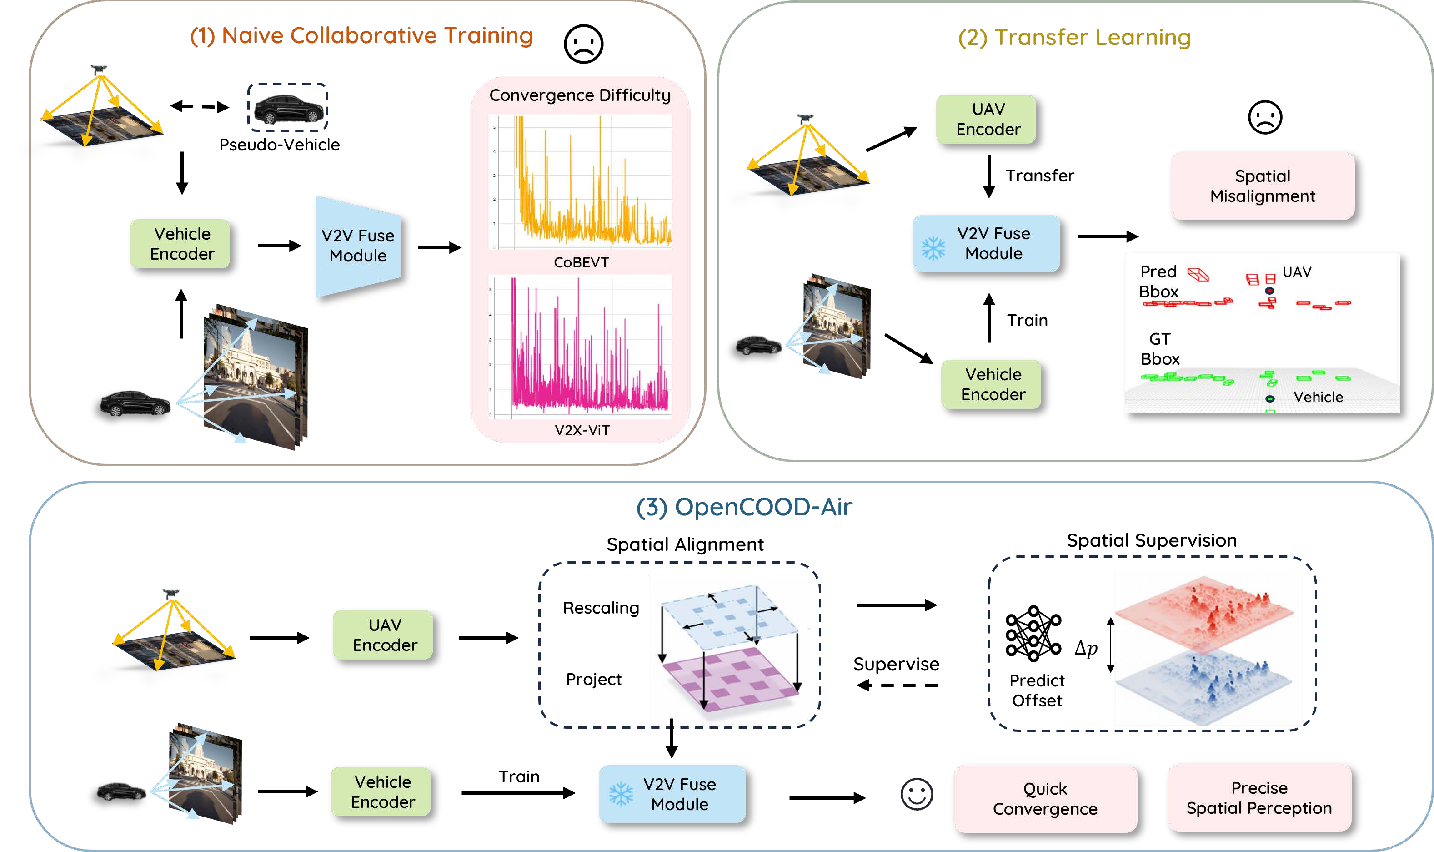
\includegraphics[width=1\textwidth]{PDF/overview.pdf}
    \caption{Overview of the OpenCOOD-Air framework and its motivation. (1) Naive Collaborative Training suffers from convergence difficulty due to the significant domain gap between ground vehicles and UAVs. (2) Transfer Learning from pre-trained V2V models stabilizes training but introduces spatial misalignment, as it fails to capture the unique altitude dimension of UAVs. (3) Our Method addresses these issues by inheriting V2V knowledge and employing a CDSC module for feature alignment, alongside a SOPT module to explicitly supervise and rectify altitude-induced geometric discrepancies.}
    \label{fig:overall_architecture}
\end{figure*}
In recent years, collaborative perception has emerged as a promising technology for autonomous driving, extending the sensing range of individual vehicles through Vehicle-to-Vehicle (V2V) communications. However, most existing frameworks are confined to the ground-level perspective. We argue that Unmanned Aerial Vehicles (UAVs) can serve as an extension of conventional V2V systems, providing a distinctive high-altitude viewpoint that helps mitigate blind spots and long-range occlusions inherent in ground-based sensors.

Despite its potential, ground-air collaborative perception faces a formidable technical challenge. The core obstacle lies in the significant domain gap and data imbalance between heterogeneous agents: while ground-level vehicle data is typically dense and shares consistent perspectives, the newly introduced UAV data is relatively sparse and captured from drastically different altitudes. This heterogeneity leads to severe gradient interference during joint training, resulting in optimization instability and poor convergence. While adopting transfer learning methods can significantly alleviate the training difficulty caused by data sparsity, it often introduces a secondary issue: since existing transfer schemes primarily focus on 2D planar features, they tend to neglect the UAV's unique altitude dimension. Consequently, vital spatial-geometric information is lost during feature transformation, limiting the performance gain of ground-air collaborative perception in complex 3D scenarios.

To address these issues, we formulate the ground-air collaborative perception problem as a heterogeneous integration task under an asymmetric cooperative paradigm, which requires explicit altitude supervision. Unlike conventional V2V systems that operate under a shared ground-plane assumption, ground-air collaborative perception must reconcile the geometric discrepancy between 2D-dominant vehicle features and 3D-expansive UAV perspectives. Specifically, we train the UAV weights based on a pre-trained V2V framework and introduce a Cross-Domain Spatial Converter (CDSC) module to facilitate cross-domain feature transformation. Furthermore, a Spatial Offset Prediction Transformer (SOPT) is designed to ensure that the CDSC and the UAV encoder capture sufficient spatial-geometric information. To evaluate our approach, we construct the OPV2V-Air dataset, a comprehensive benchmark that incorporates diverse UAV-based perspectives into existing ground-level scenarios to validate the efficacy of the transition from V2V to ground-air collaborative perception.

The main contributions of this work are as follows:
\begin{itemize}
    \item We propose OpenCOOD-Air, the first Vehicle-to-Vehicle-to-UAV(V2V2U) framework. Unlike existing studies that primarily focus on single-vehicle-to-UAV cooperation, our approach reformulates air-ground collaboration as an extension of V2V networks. OpenCOOD-Air is designed to be compatible with existing V2V architectures, providing a flexible verification platform for broader collaborative perception research.
    
    \item We design the CDSC and SOPT modules to bridge the dimensional gap between ground-air collaborative perception and traditional V2V. Unlike V2V, which operates in a near-planar dimension, our modules explicitly model the expanded vertical-spatial scale of UAVs, effectively addressing spatial misalignment and information loss caused by altitude variations.
    
    \item We introduce the OPV2V-Air dataset, which extends the OPV2V\cite{xu2022opv2v} benchmark by incorporating UAV-based perspectives to provide sufficient multi-agent data for ground-air collaborative tasks. On the OPV2V-Air dataset, our OpenCOOD-Air framework improves 2D and 3D AP@0.7 by 4\% and 7\% compared to state-of-the-art methods, respectively.
    
\end{itemize}







\begin{table}[t]
\centering
\caption{Comparison of Ground-Air Cooperative Perception Datasets}
\label{tab:comparison}
\renewcommand{\arraystretch}{1.2}
\begin{tabular*}{\columnwidth}{@{\extracolsep{\fill}}lccc@{}}
\toprule
Dataset & Mode & Max Vehicles/UAVs & Modality \\ \midrule
CoPeD \cite{zhou2024coped} & V2U & 1 / 1 & C \\
V2U-COO \cite{wang2025uvcpnet} & V2U & 1 / 2 & C \\
Griffin \cite{wang2025} & V2U & 1 / 1 & L/C \\
AGC-Drive \cite{hou2025} & V2V2U & 2 / 1 & L/C \\
AirV2X \cite{gao2025} & V2V2U & 5 / 5 & L/C \\
\textbf{OPV2V-Air(Ours)} & \textbf{V2V2U} & \textbf{7 / 7} & \textbf{L/C} \\ \bottomrule
\end{tabular*}
\end{table}
\section{Related Work}
\textbf{Collaborative Perception Datasets.}
Collaborative perception datasets have evolved from early V2V \cite{xu2022opv2v, xu2023v2v4real} configurations to more complex V2X \cite{yu2022dair, zimmer2024tumtraf, xiang2024v2x} paradigms, aiming to broaden sensing coverage through multi-agent data sharing. Recently, research has shifted towards ground-air collaboration to address persistent ground-level occlusion. V2U-COO \cite{wang2025uvcpnet} and Griffin \cite{wang2025} provide simulation-based vehicle-UAV data, while CoPeD \cite{zhou2024coped} and AGC-Drive \cite{hou2025} offer real-world multi-robot and V2V2U interactions. AirV2X \cite{gao2025} further extends this to include roadside infrastructure.

\textbf{V2X Perception.}
Collaborative perception typically follows three paradigms: early, late, and intermediate fusion \cite{8885377, 8569832, wang2020v2vnet}. Intermediate fusion has become the mainstream due to its balance between accuracy and bandwidth efficiency. Early works like F-Cooper \cite{chen2019f} and V2VNet \cite{wang2020v2vnet} utilized simple aggregations, while recent advancements such as V2X-ViT \cite{xu2022v2x} and CoBEVT \cite{xucobevt} employ Transformers to capture complex inter-agent correlations. To optimize communication, selective transmission strategies \cite{liu2020when2com, hu2022where2comm} have been proposed. For agent heterogeneity, methods like HM-ViT \cite{xiang2023hm} and STAMP \cite{gaostamp} focus on cross-modal alignment and feature normalization. Emerging LLM-based approaches \cite{gao2025langcoop, you2026v2x} further explore language as a medium for interoperability.
Among ground-air works, UVCPNet \cite{wang2025uvcpnet} pioneered vehicle-UAV collaboration but relies on fixed UAV configurations and neglects multi-vehicle coordination. In contrast, our OpenCOOD-Air framework extends V2V systems with flexible aerial perspectives, enabling robust multi-agent perception.



\section{Method}
\begin{figure*}[t]
    \centering
    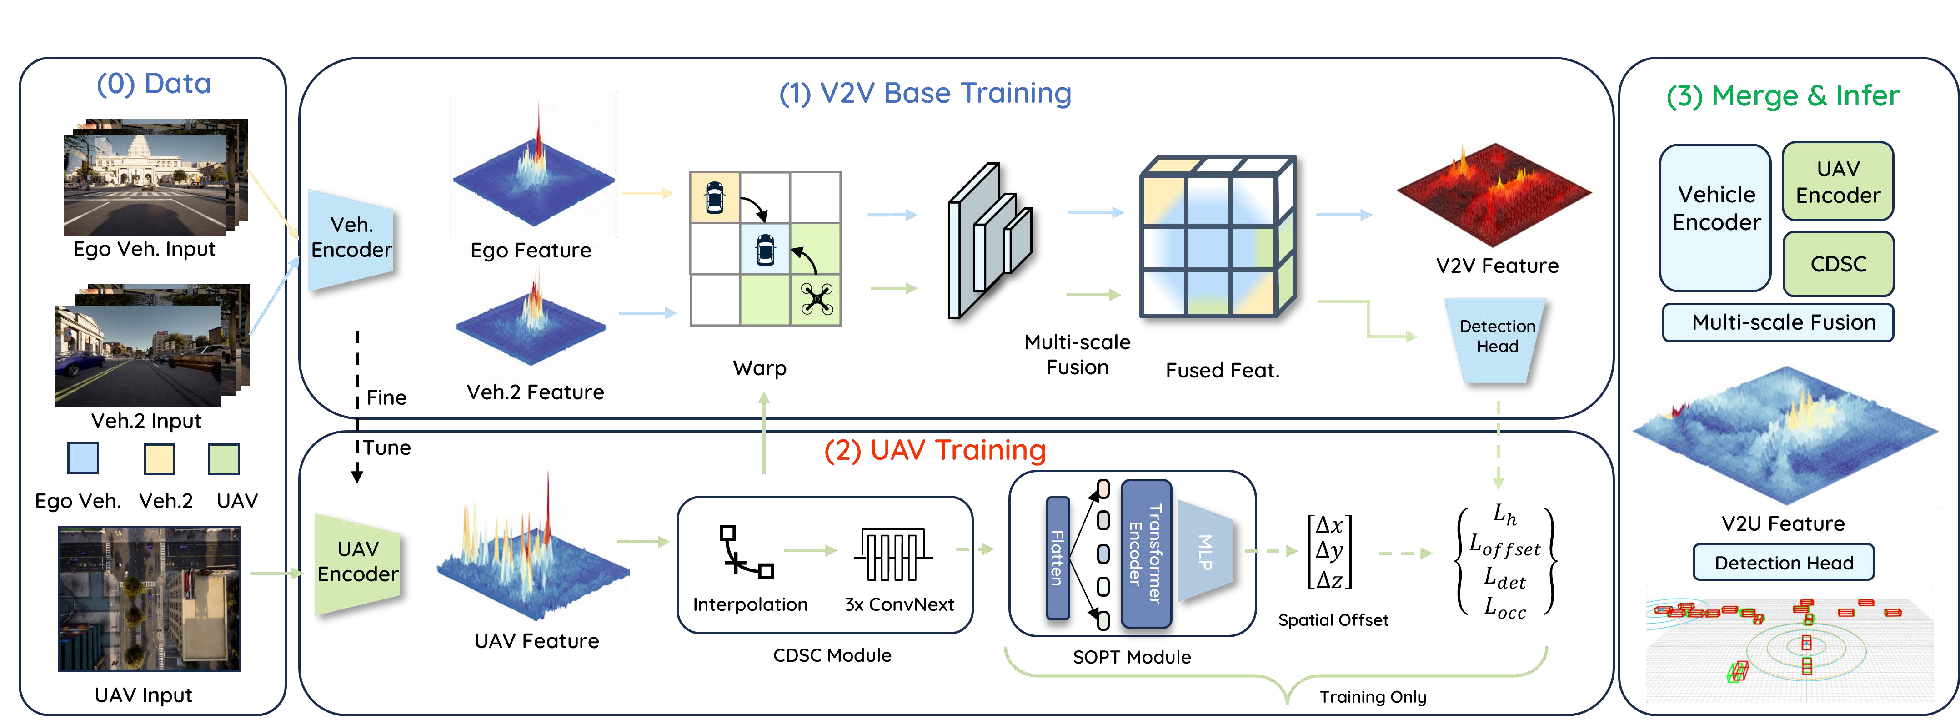
\includegraphics[width=1\linewidth]{PDF/method.pdf}
    \caption{Overview of the proposed OpenCOOD-Air framework. The architecture is implemented in three steps: (1) training base model for vehicle-to-vehicle collaboration; (2) utilizing the CDSC module and SOPT module to align aerial-ground perspectives; (3) merging trained weights and integrating V2V and V2U features for final ground-air collaborative perception.}
    \label{fig:method}
\end{figure*}

\subsection{Overview and Motivation}

The integration of UAVs into V2V networks primarily grapples with severe fusion difficulties arising from domain-heterogeneous gradients and the loss of vital spatial-geometric information during cross-view transformation. To address these challenges without incurring the prohibitive costs of end-to-end retraining, we propose a two-stage asymmetric training paradigm. We first anchor a robust V2V baseline and then freeze the fusion backbone and detection headers to serve as stable geometric references. This decoupling strategy facilitates the deployment of two specialized modules to bridge the domain gap: a CDSC module is introduced to resolve the spatial coordinate mismatch through non-linear feature alignment; additionally, a SOPT module is employed to compensate for the vertical information deficit via explicit 3D altitude supervision. By preserving pre-trained V2V knowledge while adapting to aerial perspectives, our framework achieves a seamless and stable extension from ground-only to ground-air collaborative perception.




\subsection{Cross-Domain Spatial Converter (CDSC)}
\begin{figure}[t]
    \centering
    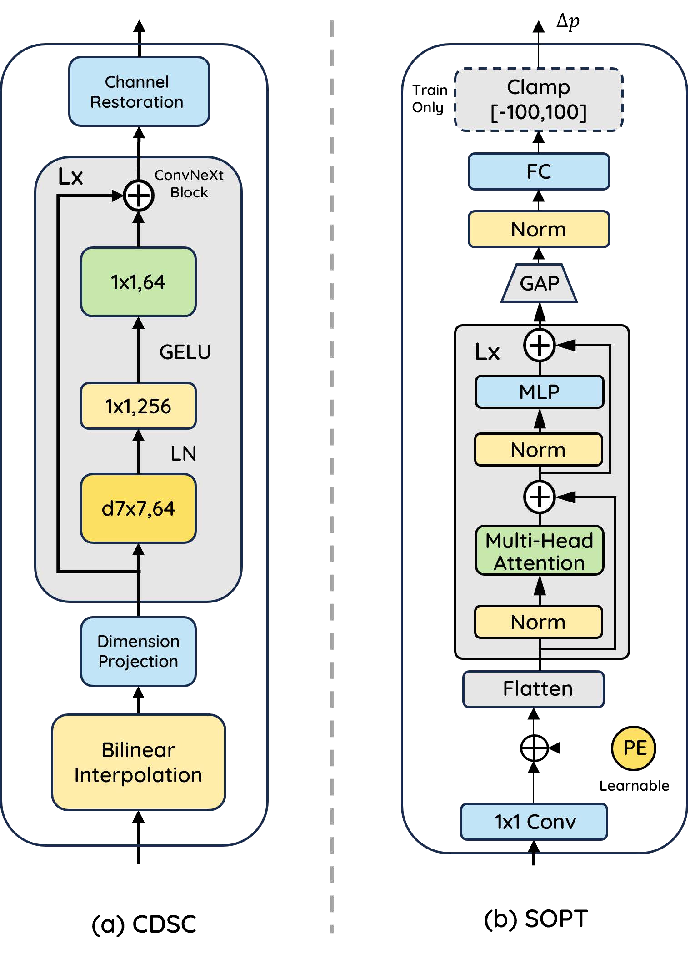
\includegraphics[width=0.9\linewidth]{PDF/CDSC_SOPT.pdf}
    \caption{Detailed architectures of the proposed modules.(a) CDSC performs spatial alignment via bilinear interpolation and ConvNeXt-based geometric rectification; (b) SOPT utilizes Transformer encoders to regress the 3D spatial offset $\Delta \mathbf{p}$ for explicit spatial supervision.}
    \label{fig:SOPT}
\end{figure}
Inspired by the adapter-based alignment in STAMP \cite{gaostamp}, we propose CDSC to tackle the specific hurdles of ground-air coordination. Unlike STAMP's focus on LiDAR-camera fusion, our task relies solely on visual input, where the primary challenge lies in the vast perspective disparity between UAVs and ground vehicles. CDSC effectively rectifies high-altitude UAV features into a standardized spatial coordinate system, enforcing geometric consistency essential for heterogeneous agent collaboration.


\subsubsection{Resolution Rescaling}
The CDSC first addresses the spatial resolution mismatches by calculating a spatial scaling factor based on the physical scale difference between the UAV-side feature maps and the target collaborative BEV space. Bilinear interpolation is employed to resample the input features to the target resolution:
\begin{equation}
F'_{\text{in}} = \mathcal{I}(F_{\text{in}}, \lambda)
\end{equation}
where $F_{\text{in}}$ denotes the raw feature map from the UAV encoder, $\mathcal{I}(\cdot)$ represents the bilinear interpolation function, and $\lambda$ is the scaling coefficient derived from the ratio of the target V2V resolution to the UAV resolution

\subsubsection{Cross-Domain Feature Mapping}
Following resolution rescaling, we employ a ConvNeXt-based~\cite{liu2022convnet} architecture to execute spatial mapping and mitigate the domain gap. ConvNeXt's large-kernel design is particularly suitable for this task, as it enables expanded receptive fields for global contextual integration and  effective geometric rectification without introducing excessive parameters. The conversion process is formulated as:
\begin{equation}
F_{\text{out}} = \phi_{\text{out}}\left(\Psi\left(\phi_{\text{in}}(F'_{\text{in}})\right)\right)
\end{equation}
where $\phi_{\text{in}}$ is a $1 \times 1$ convolution used to project features into the hidden layer dimension; $\Psi(\cdot)$ represents a sequence of ConvNeXt blocks, and $\phi_{\text{out}}$ is a $1 \times 1$ convolution that maps the features to the required target channel count $C_{\text{out}}$.

By expanding the receptive field, this process integrates extensive spatial contextual information into the feature maps, shifting the focus from ground vehicles to a high-dimensional semantic perception of the overall ground environment. The transformed features become more robust to the Z-axis distribution shift while maintaining compatibility with the pre-trained V2V perception logic and are subsequently processed by the SOPT module for explicit geometric offset prediction.



\subsection{SOPT: Spatial Offset Prediction Transformer}
To provide explicit geometric constraints during training without increasing inference latency, we design the SOPT module as an auxiliary supervision branch. This module is active only during the second training stage to force the upstream CDSC to internalize spatially aware representations. Implicitly, this predictive task forces the backbone to preserve spatial geometry information, effectively filtering out environmental noise. Based on this representation, the model explicitly predicts the 3D spatial offset of the UAV relative to the standard V2V coordinate system.

\subsubsection{Feature Projection and Tokenization}
To reduce computational complexity and achieve cross-channel feature aggregation while preserving spatial topology, we project the features from the CDSC into a latent embedding space and incorporate positional information. The initial token sequence $\mathbf{X}_0$ is formulated as:
\begin{equation}
\mathbf{X}_0 = \text{Flatten}\left( \text{Proj}(\mathbf{F}_{\text{out}}) + \mathbf{E}_{\text{pos}} \right)
\end{equation}
where $\mathbf{F}_{\text{out}} \in \mathbb{R}^{C \times H \times W}$ denotes the features from the CDSC, and $\text{Proj}(\cdot)$ denotes a linear projection that aligns the channel dimension $C$ with the transformer embedding dimension $D$. $\mathbf{E}_{\text{pos}} \in \mathbb{R}^{D \times H \times W}$ is a 2D learnable positional encoding introduced to retain spatial structural information. After the flattening operation, the resulting sequence $\mathbf{X}_0 \in \mathbb{R}^{HW \times D}$ represents each grid cell in the BEV map as a discrete token, providing the fundamental primitives for subsequent global modeling.

\subsubsection{Global Context Encoding} 
To mitigate non-linear scaling and perspective distortions induced by viewpoint height variations, we deploy $L$ layers of Transformer encoders to establish long-range geometric constraints. This module captures long-range correlations between tokens across the entire map via a Multi-Head Self-Attention (MSA) mechanism, with the update logic for each layer $l \in \{1, \dots, L\}$ formulated as:
\begin{align}
    \mathbf{X}_l' &= \text{MSA}(\text{LN}(\mathbf{X}_{l - 1})) + \mathbf{X}_{l - 1}, \\
    \mathbf{X}_l &= \text{FFN}(\text{LN}(\mathbf{X}_l')) + \mathbf{X}_l',
\end{align}
where $\mathbf{X}_{l-1}$ and $\mathbf{X}_{l}$ represent the input and output token sequences of the $l$-th layer, respectively. $\text{LN}(\cdot)$ denotes Layer Normalization, and $\text{FFN}(\cdot)$ represents the Feed-Forward Network. Through this hierarchical information exchange, the model effectively identifies and compensates for systematic distribution biases caused by height differences, resulting in a more robust global representation.

\subsubsection{Offset Regression}
To obtain a compact global descriptor and predict the spatial displacement between viewpoints, we aggregate the deep global representation and map it to a translation vector. To ensure training stability and prevent gradient instability in the early stages, the 3D spatial offset $\Delta \mathbf{p}$ is regressed via an MLP and subsequently constrained by a clipping function:
\begin{align}
    \Delta \mathbf{p}_{\text{raw}} &= \text{MLP}(\text{LN}(\text{GAP}(\mathbf{X}_L))), \\
    \Delta \mathbf{p} &= \text{Clamp}(\Delta \mathbf{p}_{\text{raw}}, -\tau_c, \tau_c),
\end{align}
where $\mathbf{X}_L$ is the final output sequence of the encoder, $\text{GAP}$ and $\text{LN}$ denote Global Average Pooling and Layer Normalization, respectively, and $\tau_c$ is a predefined clipping threshold from the perception range. The resulting vector $\Delta \mathbf{p} = (\Delta x, \Delta y, \Delta z)$ quantifies the 3D translation offset of the UAV viewpoint relative to the ego-vehicle in a unified BEV world coordinate system. The predicted vector $\Delta \mathbf{p}$ is utilized solely to compute the offset loss $\mathcal{L}_{\text{offset}}$. The resulting gradients propagate back to the CDSC and encoder, effectively anchoring the latent feature space to physical geometric dimensions. Once training is complete, SOPT is discarded, leaving a computationally efficient and spatially calibrated backbone for deployment.



\subsection{Joint Optimization Objectives}

\subsubsection{Feature Offset Supervision}

To ensure that the regressed translation vector accurately captures the spatial relationships between viewpoints and to prevent representation drift during training, we introduce a global offset regression loss $\mathcal{L}_{\text{offset}}$. Specifically, we employ the Smooth-L1 objective function, utilizing the ground truth $\Delta \mathbf{p}_{\text{gt}}$ derived from sensor extrinsics to supervise the predicted offset $\Delta \mathbf{p}$:

\begin{equation}
\mathcal{L}_{\text{offset}} = \text{SmoothL1}(\Delta \mathbf{p}, \Delta \mathbf{p}_{\text{gt}})
\end{equation}
where $\Delta \mathbf{p}_{\text{gt}}$ represents the target 3D spatial displacement. This explicit geometric constraint guides the SOPT module to maintain a consistent understanding of 3D poses while simultaneously guiding the CDSC module to learn more effective spatial alignment mappings. 

By anchoring the feature transformation to physical spatial constraints, the model avoids the local minima often associated with purely appearance-based feature matching, ensuring more robust convergence during the second-stage training.

\subsubsection{Height Calibration and Vertical Consistency Loss}

To explicitly supervise the UAV's capability in predicting the height of ground objects, we introduce a vertical consistency loss $\mathcal{L}_{z\_\text{align}}$. For the set of positive samples $\mathcal{P}$, the objective is defined as the mean absolute error between the predicted height and the ground truth.

However, during the second-stage training, since the regression weights of the detection head are fixed to ground-level statistics, the significant Out-of-Distribution (OOD) shift of the UAV relative to the ground coordinate system exceeds its mapping capacity. This often leads to 3D localization failure along the $Z$-axis. To eliminate the systematic absolute numerical bias along the $Z$-axis and align the predicted targets with the ground coordinate system, we perform a macro-adjustment via physical calibration during training. Following the anchor-normalized parametrization common in 3D detection, the calibrated center height residual $\hat{t}_{z}^{\text{final}}$ is formulated as:
\begin{equation}
\hat{t}_{z}^{\text{final}} = \hat{t}_{z}^{\text{raw}} - \frac{\Delta z}{h_{\text{anchor}}}
\end{equation}
where $\hat{t}_{z}^{\text{raw}}$ is the raw $Z$-axis regression output from the detection head, and $h_{\text{anchor}}$ denotes the predefined anchor height. The correction term $\Delta z$ is the height component extracted from the predicted 3D offset vector $\Delta \mathbf{p}$. Physically, this operation compensates for the systematic height deviation of the predicted box center, effectively shifting the global geometric structure back to the baseline coordinate system.

On this basis, we define the vertical geometric consistency loss $\mathcal{L}_{z\_\text{align}}$ as:

\begin{equation}
\mathcal{L}_{z\_\text{align}} = \frac{1}{|\mathcal{P}|} \sum_{i \in \mathcal{P}} |z_{\text{pred}}^{(i)} - z_{gt}^{(i)}|
\end{equation}
where $z_{\text{pred}}^{(i)}$ and $z_{\text{gt}}^{(i)}$ denote the calibrated predicted center height and the corresponding ground truth height for the $i$-th sample, respectively, and $|\mathcal{P}|$ represents the number of positive samples.

Notably, the gradients from $\mathcal{L}_{z\_\text{align}}$ and $\mathcal{L}_{\text{offset}}$ enable the CDSC to produce features that are already height-compensated, thereby ensuring that the transformed features are spatially consistent for subsequent pyramid fusion.



\section{Experiment}
\subsection{Dataset: OPV2V-Air}

% 保持原图位置
\begin{figure}[t]
    \centering
    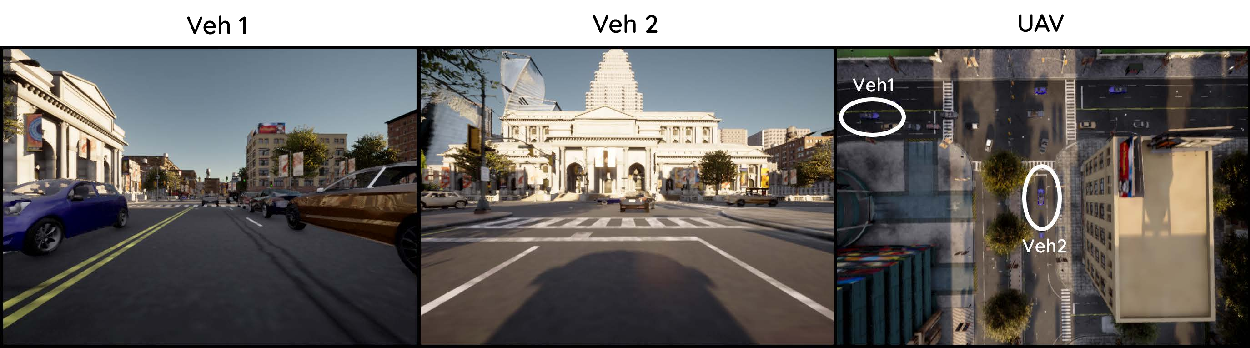
\includegraphics[width=0.48\textwidth]{PDF/data_example_mini.pdf} 
    \caption{Camera data examples of the OPV2V-Air dataset. The white circle highlight the position of Vehicle 1 and Vehicle 2 in the data of UAV. }
    \label{fig:visualization_samples}
\end{figure}

To evaluate the transition from V2V to ground-air collaborative perception, we conduct experiments on our self-collected OPV2V-Air dataset. This benchmark is constructed by replaying 68 scenarios from OPV2V \cite{xu2022opv2v} across eight CARLA towns (Town01--07, 10) via the OpenCDA \cite{xu2021opencda} platform. By strictly following original vehicle trajectories, we extend the ground-only paradigm to an ground-air setting while preserving multi-agent spatial dynamics (Fig.~\ref{fig:visualization_samples}).

\textbf{Sensor Configurations.}
The sensor suite is designed for multi-modal and visibility-aware perception. Specifically, each ground vehicle is equipped with 4$\times$ RGB and 4$\times$ Depth cameras (Res: $800 \times 600$, FOV: $100^\circ$) and a 64-channel LiDAR (V-FOV: $[$-$30^\circ, 10^\circ]$). The UAV operates at an altitude of \SI{50}{\metre}, carrying 1$\times$ RGB and 1$\times$ Depth camera (Res: $800 \times 600$) along with a 64-channel LiDAR featuring a downward-facing V-FOV of $[$-$90^\circ, $-$30^\circ]$. During training, we utilize visibility-aware BEV maps to filter out-of-range vehicles and employ depth maps for depth supervision.

\textbf{Annotation and Tasks.}
The dataset provides high-fidelity ground truth, including 3D bounding boxes, LiDAR point clouds, and visibility-aware BEV maps. In this study, we utilize visibility BEV maps from OpenCDA to filter out-of-range vehicles and ensure label reliability.


\subsection{Implementation Details}
All models were trained for 50 epochs on a server equipped with two NVIDIA GeForce RTX 4090 GPUs. We utilized the Adam optimizer with an initial learning rate of 0.001, combined with a MultiStepLR scheduler that decays the learning rate by a factor of 0.1 at the 20th and 40th epochs. 

During the first stage of training, we utilize Pyramid Fusion as the fusion backbone, training exclusively on the vehicle-side data.. The spatial coordinates are defined within the range of $x, y \in [-51.2\,\text{m}, 51.2\,\text{m}]$ and $z \in [-3\,\text{m}, 1\,\text{m}]$. In the second stage, we leverage the UAV-side data, and the vertical training range is extended to $z \in [-60\,\text{m}, 10\,\text{m}]$. Building upon the weights optimized in the first stage, we freeze the V2V fusion backbone and detection head, and jointly train the UAV Encoder, CDSC, and SOPT modules. 

During inference, the trained CDSC and the fine-tuned Encoder are integrated into the V2V cooperative perception framework, forming dual feature processing paths for vehicle and UAV inputs, respectively. After feature extraction and alignment, features from both sources are fused and passed to the detection heads to complete the ground-air object detection task.


\subsection{Evaluation Metrics}To comprehensively evaluate perception performance, we employ both 2D and 3D Average Precision (AP) as primary metrics.
\subsubsection{2D Evaluation}
Following the OPV2V \cite{xu2022opv2v} protocol, 3D bounding boxes are projected onto the BEV plane to evaluate horizontal localization.
\subsubsection{3D Evaluation}
Considering the significant altitude disparity in ground-air scenarios, we introduce a rotation-aware volumetric 3D IoU to measure vertical alignment precision. Utilizing the Shapely library for oriented polygon intersection, the 3D IoU is defined as:
\begin{equation}
\text{IoU}_{\text{3D}} = \frac{\text{Area}(\mathcal{P}_p \cap \mathcal{P}_g) \times \Delta z}{V_p + V_g - V_{\text{inter}}}
\end{equation}
where $V_p$ and $V_g$ are the volumes of the boxes, and $V_{\text{inter}}$ denotes the intersection volume. The term $\Delta z$ represents the overlap height along the $Z$-axis, formulated as $\Delta z = \max(0, \min(z_{max,p}, z_{max,g}) - \max(z_{min,p}, z_{min,g}))$.


\subsection{Quantitative Results}
\subsubsection{Baseline Comparison}

\begin{table}[t]
\centering
\caption{Quantitative comparison and model complexity on OPV2V-Air. AP is evaluated at IoU=0.7. 'Params' denotes the total number of trainable parameters.}
\label{tab:eval_results}
\begin{tabular*}{\columnwidth}{@{\extracolsep{\fill}}lccc@{\extracolsep{\fill}}}
\toprule
Method & Params (M) $\downarrow$ & 2D Eval. $\uparrow$ & 3D Eval. $\uparrow$ \\
\midrule
Ours (Vehicles) & - & 39 & 27 \\
\midrule
V2X-ViT \cite{xu2022v2x} & 36.53 & 15 & 7 \\
CoBEVT \cite{xucobevt} & 33.61 & 33 & 16 \\
Where2comm \cite{hu2022where2comm} & 31.53 & 41 & 23 \\
V2VNet \cite{wang2020v2vnet} & 37.69 & 66 & 50 \\
HEAL \cite{luextensible} & \textbf{15.02} & 67 & 44 \\
\textbf{OpenCOOD-Air(ours)} & 20.33 & \textbf{71} & \textbf{57} \\
\bottomrule
\end{tabular*}
\end{table}

Due to the scarcity of open-source frameworks specifically designed for ground-air collaborative perception, we evaluate our method by adapting five SOTA V2V models: CoBEVT, Where2comm, V2X-ViT, V2VNet, and HEAL. These methods, while highly effective in V2V scenarios, often struggle with the drastic perspective shifts and heterogeneous coordinate transformations inherent in ground-air coordination. For a consistent evaluation, all baselines are configured with a collaborative setup of three vehicles and two UAVs. In our experimental setup, each UAV is treated as a collaborative pseudo-vehicle within the V2V framework. Furthermore, we designed a "Vehicles" experiment, which runs in the same network as our OpenCOOD-Air framework but only contains the vehicles, to quantify the performance of the ground modality independently and highlight the collaborative gain achieved by our framework in bridging the spatial domain gap.

The quantitative results in Table \ref{tab:eval_results} further demonstrate the superiority of our approach. First, compared to the Ours-Vehicles baseline, methods such as V2X-ViT and CoBEVT suffer severe performance degradation upon integrating UAV data, highlighting the vulnerability of existing models to ground-air heterogeneous data. When compared with stronger SOTA models: in the 2D dimension, our method maintains a 4\% lead in AP@0.7 even over HEAL; in the more challenging 3D dimension, compared to the top-performing V2VNet, our method achieves a 7\% gain in 3D AP@0.7. This indicates that our framework outperforms existing methods in both BEV horizontal localization and vertical spatial alignment.

In terms of model complexity, OpenCOOD-Air achieves a superior performance-efficiency trade-off. Although slightly larger than HEAL, our method yields a 7\% 3D AP gain with minimal parameter overhead. Furthermore, it outperforms other SOTA methods like V2VNet while reducing the parameter count by nearly 40\%, demonstrating the effectiveness of our decoupled transfer learning strategy and the lightweight design of CDSC and SOPT modules.

\begin{table}[t]
\centering
\caption{2D Detection Performance (AP@0.7) Across Vehicle-UAV Combinations}
\label{tab:combination}
\renewcommand{\arraystretch}{1.2} 
\begin{tabular}{>{\centering\arraybackslash}p{1.6cm} | >{\centering\arraybackslash}p{1.8cm} >{\centering\arraybackslash}p{1.8cm} >{\centering\arraybackslash}p{1.8cm}}
\toprule
Veh. \textbackslash{} UAV & 0 & 1 & 2 \\ \midrule
1 & 10 & 47 & 63 \\
2 & 29 & 59 & 70 \\
3 & 39 & 63 & 71 \\ \bottomrule
\end{tabular}
\end{table}
\subsubsection{Effectiveness of Agent Combinations}
Table~\ref{tab:combination} presents the detection performance under common vehicle-UAV combinations in the OPV2V-Air dataset. The data reveal that heterogeneous integration provides a more substantial boost than simply increasing ground agents. Notably, the 1V+1U configuration outperforms the 3V-only baseline, suggesting that viewpoint diversity is more effective than increasing ground-level agent density. This discrepancy is likely due to the inherent limitations of horizontal viewpoints in occluded environments. While adding more vehicles yields incremental gains, the integration of a UAV provides coverage of ground-level blind spots, leading to a more substantial performance leap.Furthermore, while the system exhibits robust scalability, we observe diminishing marginal returns as the fleet expands, indicating that the aerial perspective provides rapid but eventually saturating coverage of the environment.


\subsubsection{Robustness Analysis}
\begin{figure}[t]
    \centering
    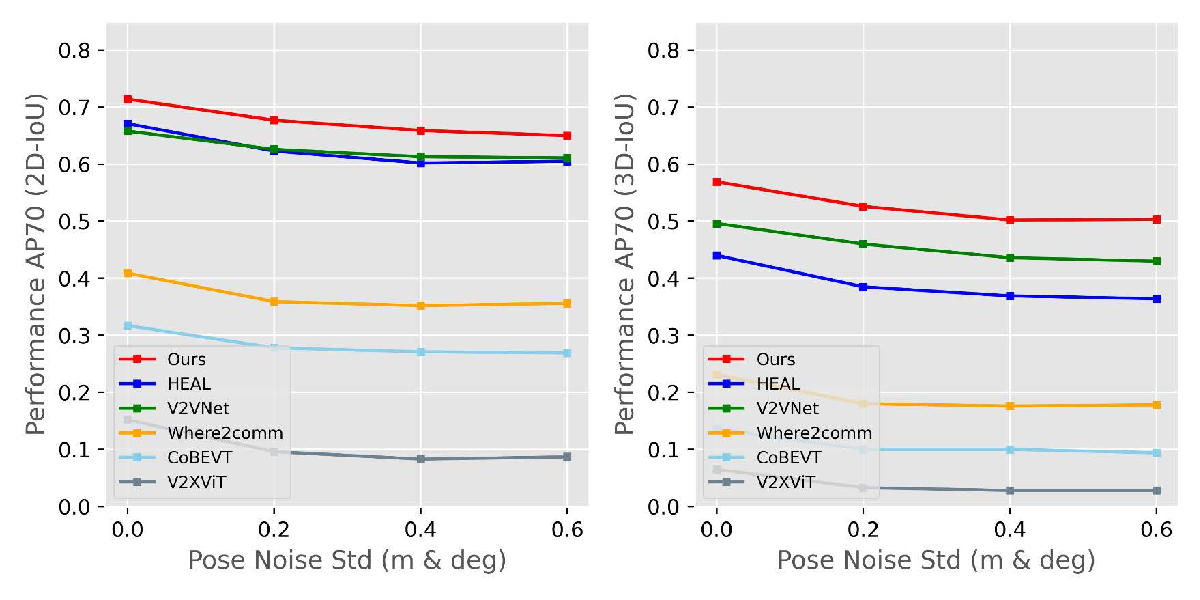
\includegraphics[width=1\linewidth]{PDF/noise_only.pdf}
    \caption{Robust Experiment to pose error. Pose noise is set to $\mathcal{N}(0, \sigma_p^2)$ on x, y location and $\mathcal{N}(0, \sigma_r^2)$ on yaw angle.}
    \label{fig:noise_param}
\end{figure}

\begin{table}[t]
\centering
\caption{Impact of Compression Rate on Detection Performance (AP@0.7).}
\label{tab:compression}
\renewcommand{\arraystretch}{1.3}
\setlength{\tabcolsep}{17pt}
\begin{tabular}{c | c c}
\toprule
Compression Rate & 2D Eval.  $\uparrow$ & 3D Eval.  $\uparrow$ \\
\midrule
Original & 71 & 57 \\
4$\times$ & 67 & 51 \\
8$\times$ & 66 & 50 \\
16$\times$ & 64 & 45 \\
64$\times$ & 42 & 24 \\
\bottomrule
\end{tabular}
\end{table}

To assess system reliability under real-world localization inaccuracies, we introduce synthetic pose noise with standard deviations ranging from 0.0 to 0.6 (meters and degrees). As illustrated in Fig. \ref{fig:noise_param}, while baseline methods suffer significant performance degradation due to spatial misalignment, our framework demonstrates superior robustness. Specifically, even at the highest noise level, our method retains over 90\% of its original performance, consistently outperforming the second-best method by a substantial margin.


\subsubsection{Compression Rate Analysis}
As shown in Table~\ref{tab:compression}, at 16$\times$ compression, our method surpasses V2X-ViT, CoBEVT, and Where2comm without compression. Even at 64$\times$ compression, basic detection capability is preserved, validating robustness for bandwidth-constrained scenarios.




\subsection{Ablation Study} We conducted ablation experiments on the OPV2V-Air dataset to evaluate the effectiveness of the CDSC and SOPT modules. The results, summarized in Table \ref{tab:ablation_study}, demonstrate that both modules contribute significantly to the overall performance through distinct functional roles.

The CDSC exhibits potent spatial alignment capabilities; upon its integration, the model's 2D AP@0.7 performance improves by 4\% and reaches a plateau. However, a performance gap persists in high-precision 3D metrics, where the 3D AP@0.7 remains at 44. By introducing the SOPT module to provide explicit spatial supervision, the model's predictive accuracy in the high-precision 3D AP@0.7 metric improves substantially from 44 to 57, representing a 29.5\% relative gain. 
\begin{table}[t]
\centering
\caption{Ablation Study of CDSC and SOPT}
\label{tab:ablation_study}
\resizebox{\columnwidth}{!}{% 强制缩放到单栏宽度
\renewcommand{\arraystretch}{1.2} % 与前表统一的行高
\begin{tabular}{llcccc}
\toprule
\multirow{2}{*}{CDSC} & \multirow{2}{*}{SOPT} & \multicolumn{2}{c}{2D Eval.}$\uparrow$ & \multicolumn{2}{c}{3D Eval.}$\uparrow$ \\ 
\cmidrule(lr){3-4} \cmidrule(l){5-6} 
 & & AP@0.5 & AP@0.7 & AP@0.5 & AP@0.7 \\ \midrule
% Baseline
$-$ & $-$ & 78 & 67 & 71 & 44 \\ 
% 只有 SOPT
$-$ & \checkmark & 78 & 69 & 72 & 55 \\ 
\checkmark & $-$ & \textbf{83} & \textbf{71} & 75 & 44 \\ 
% Full Model
\checkmark & \checkmark & \textbf{83} & \textbf{71} & \textbf{76} & \textbf{57} \\ 
\midrule

\end{tabular}%
}
\end{table}




\subsection{Qualitative Visualizations}
\begin{figure}[t]
    \centering
    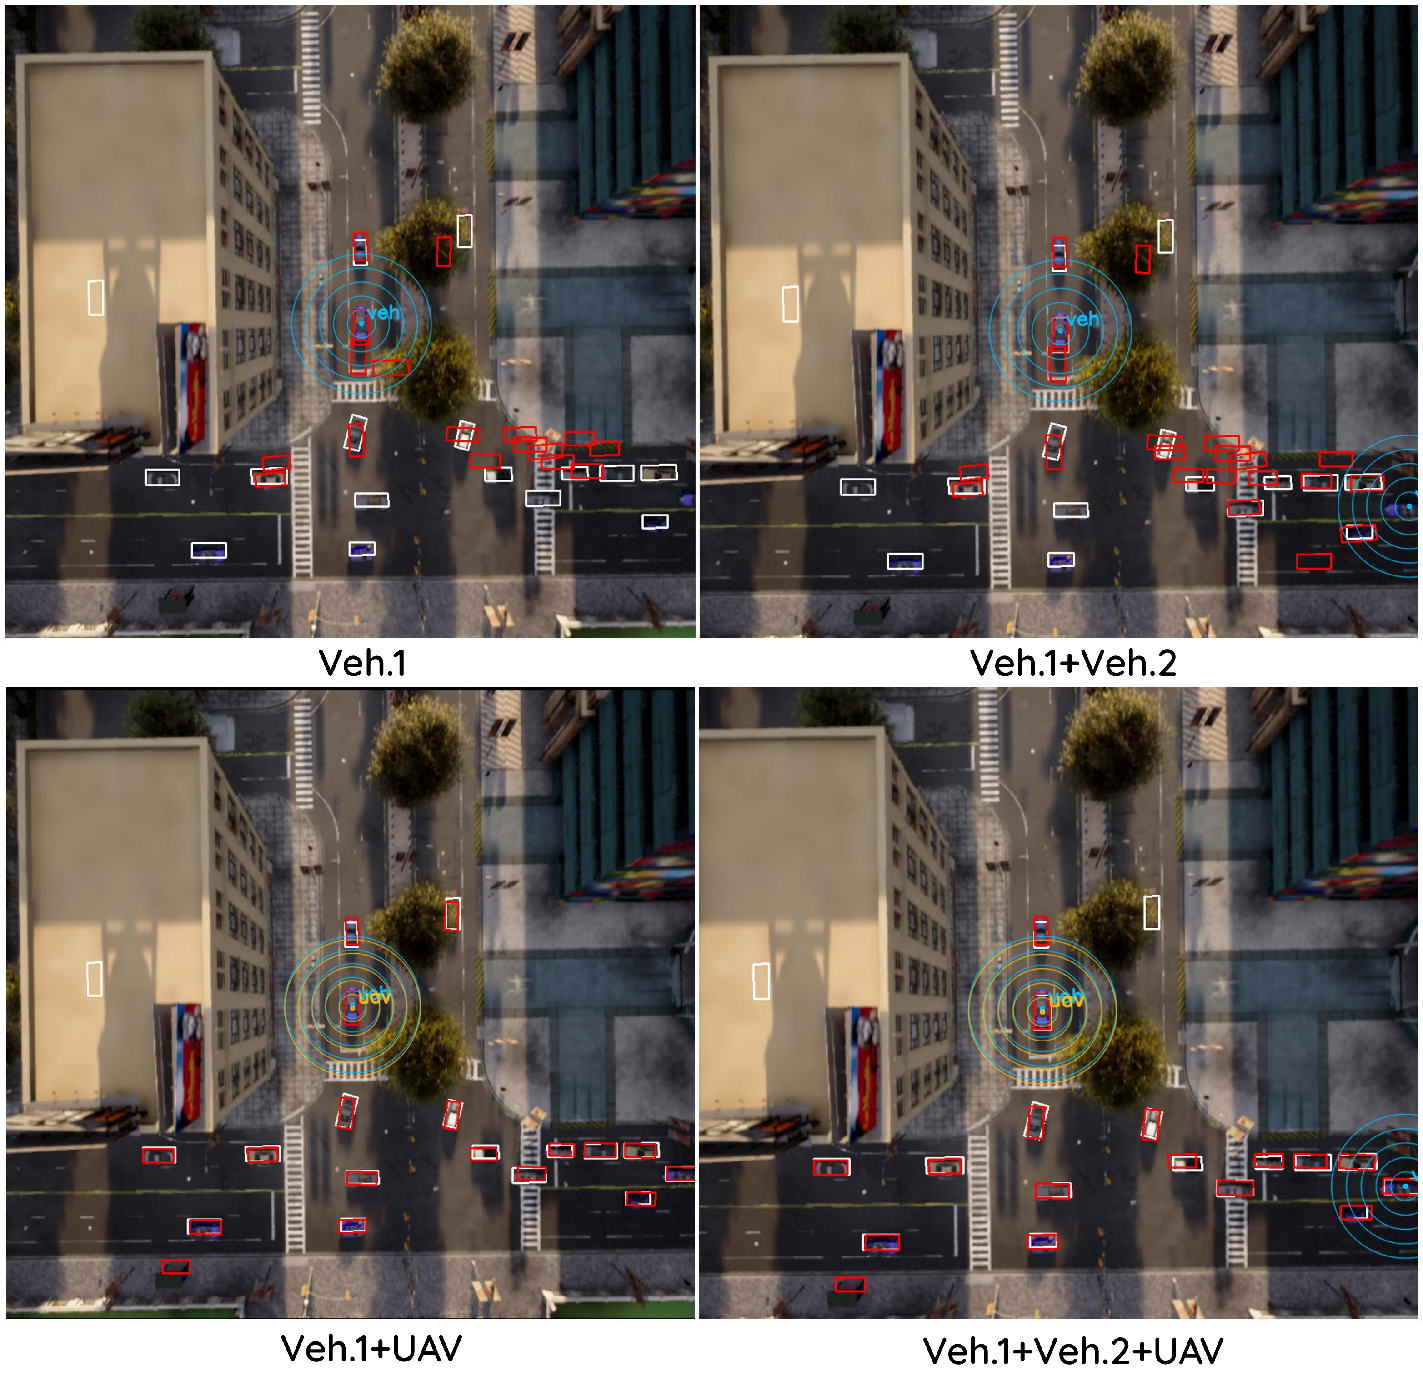
\includegraphics[width=1\linewidth]{PDF/Comparison.pdf}
    \caption{Qualitative results of progressive multi-agent collaborative perception: from single-vehicle to V2V2U.}
    \label{fig:Comparison}
\end{figure}
\begin{figure}[t]
    \centering
    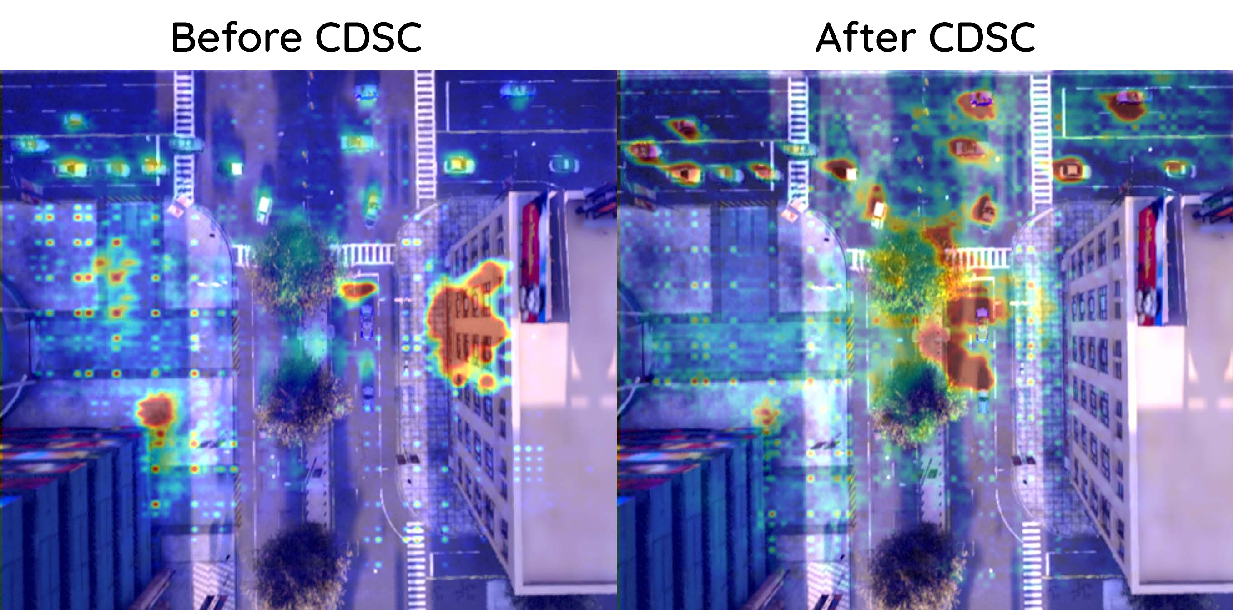
\includegraphics[width=1\linewidth]{PDF/qual-vis.pdf}
    \caption{Qualitative visualizations of the impact of CDSC module.}
    \label{fig:qual-vis}
\end{figure}


Fig.~\ref{fig:Comparison} illustrates the incremental performance gains across different configurations. In the single-vehicle setup, perception is limited by urban occlusions and narrow fields of view. While V2V communication (Veh.1+Veh.2) extends the sensing range, ground-level perspectives still struggle with distant or heavily occluded targets. By integrating a UAV (Veh.1+Veh.2+UAV), the system achieves higher precision through complementary bird’s-eye-view (BEV) information without disrupting the existing V2V logic. Similarly, adding a second vehicle to a single-vehicle-UAV pair further expands local coverage.

Fig.~\ref{fig:qual-vis} illustrates the visual impact of the CDSC on UAV feature representations. In the baseline configuration, perception is often hindered by complex environmental noise and dimensional disparities. As shown, the features from the standard encoder are heavily diffused by irrelevant background noise. By incorporating the explicit spatial guidance, the model effectively bypasses environmental clutter and achieves precise object-level focus. 



\section{Conclusion}
In this paper, we presented OpenCOOD-Air, a novel and extensible ground-air collaborative perception framework that seamlessly integrates UAVs into existing V2V systems. By addressing the fundamental challenges of domain gaps and spatial misalignment between heterogeneous agents, we formulated the collaboration as a 3D-aware integration task. Our approach leverages a two-stage hybrid adaptation strategy to mitigate gradient interference while preserving spatial-geometric integrity through the proposed CDSC and SOPT modules. To facilitate research in this domain, we introduced the OPV2V-Air benchmark, providing a comprehensive data foundation for V2V-to-V2V2U transitions. Experimental results demonstrate that OpenCOOD-Air not only significantly enhances 3D detection accuracy in occluded and long-range scenarios but also achieves superior efficiency in terms of training time and parameter optimization. Future work will explore the scalability of OpenCOOD-Air in more complex, dynamic urban environments with higher agent densities.


% \section*{References}



\bibliographystyle{IEEEtran} % 设置 IEEE 官方样式
\bibliography{ref}       % 导入你的 dataset.bib 文件
\vspace{12pt}


% \appendix
% \section{Experiments Results}





\end{document}
